\section{Sequentielle Realisierung}
Unser erster Schritt zu einem parallel berechneten Pythagoras-Baum war die serielle Umsetzung des Algorithmus, welche
uns bereits aus Programmiertechnik 2 bei Prof.~Bittel bekannt war. 

\vspace{-0.25cm}
\subsubsection*{Klassen}
\vspace{-0.25cm}
Um eine möglichst übersichtliche Projektstruktur zu erhalten, entschieden wir uns für eine Implementierung, bei der die einzelnen 
Bestandteile unseres Baums (Punkte, Quader, Dreiecke) als Klassen realisiert wurden.
Dabei definierten wir unser dreidimensionales \hyperref[Koordinatensystem]{Koordinatensystem} und einigten uns auf eine einheitliche
Benennungen der Ecken und Kanten unserer \hyperref[Koerper]{Körper}.

\vspace{-0.25cm}
\subsubsection*{Verschiebung der Objekte im Raum}
\vspace{-0.25cm}
    Die größte Herausforderung in der sequentiellen Umsetzung des Pythagoras-Baums bestand darin, die verschiedenen Komponenten korrekt 
    zu platzieren. Anders als im zweidimensionalen Raum kann der Punkt C des Dreiecks, welches auf der vorderen oberen Kante des Quaders 
    aufgesetzt wird, im Dreidimensionalen nicht einfach berechnet werden. \\
\begin{minipage}{0.3\linewidth}
    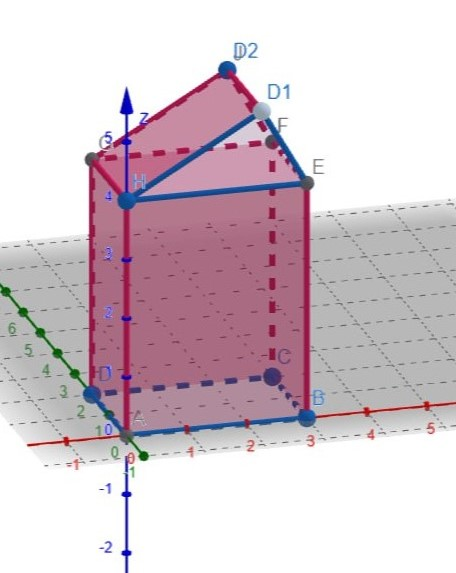
\includegraphics[width=\linewidth]{./pictures/Dreiecksberechnung_Geogebra.jpg}
    %\caption{Zu bestimmender Punkt - Geogebra}
\end{minipage}
\hfill
\begin{minipage}{0.68\linewidth}
    Unser erster Ansatz war das Umstrukturieren unserer im Zweidimensionalen funktionalen Methode zu einer im dreidimensionalen wirksamen 
    Funktion. Nach einiger Zeit stellte sich jedoch heraus, dass dies programmatisch und auch mathematisch in dieser Form nicht möglich ist.
\end{minipage}

\vspace{0.5cm}
\noindent
In Folge dessen entschieden wir uns für eine Lösung mit Transformationsmatrizen. Während wir die Seitenlänge eines neuen
Quaders weiterhin über trigonometrische Berechnungen bestimmten, wurde nun jeder neue Quader mit Ecke A im Koordinatenursprung (0|0|0) 
erzeugt. Anschließend wurde jeder Punkt einzeln mit Hilfe einer Rotationsmatrix an seine neue Position gedreht und um einen 
Vektor an die richtige Stelle im Koordinatensystem verschoben.

\noindent
\begin{figure}[h!]
    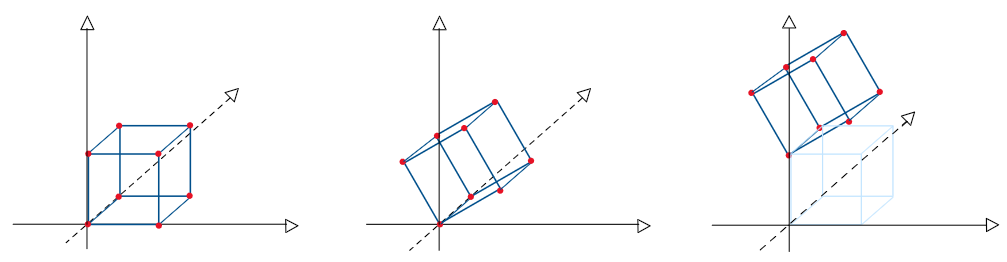
\includegraphics[width=\linewidth]{./pictures/Wuerfeltransformation.PNG}
    \caption{Transformation eines Quaders}
\end{figure}

% ----------------------------------- Rekursion ---------------------------------------
% ----------------------------------------------------------------------------------
\subsection{Rekursion}
\vspace{-0.25cm}
\begin{minipage}{0.59\linewidth}
    Der einfachste Weg zur Erzeugung eines Pythagoras-Baums, welcher uns bereits aus Programmiertechnik 2 bekannt war,
    ist eine rekursive Funktion. Diese ist so strukturiert, dass zu Beginn geprüft wird, ob die Abbruchbedingung erfüllt 
    ist. Falls ja, wird die Rekursion beendet. Anderenfalls wird die Seitenlänge des neuen Quaders berechnet. Anschließend
    ruft die Funktion sich mit ebendieser Länge selbst wieder auf.\\
    Diesem Ansatz entsprechend haben wir die Funktion \texttt{buildTree()} implementiert, bei welcher eine vorab festgelegte
    minimale Seitenlänge als Abbruchbedingung zum Einsatz kam.     
\end{minipage}
\hfill 
\begin{minipage}{0.39\linewidth}
    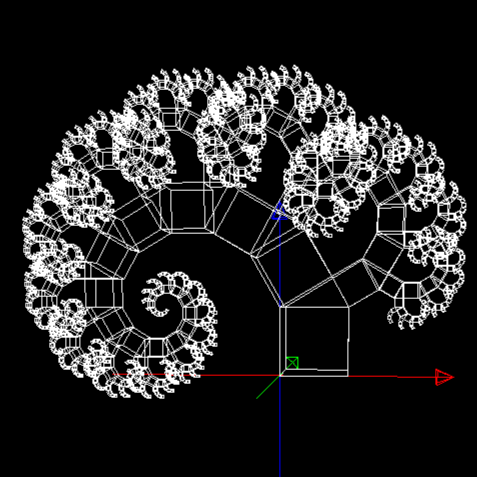
\includegraphics[width=\linewidth]{./pictures/seriell-fixed_0.1.PNG}
    \captionof{figure}{Pythagoras-Baum. \\Minimale Seitenlänge: 0.1, Winkel $\alpha$: 30°}
    \label{fig:BaumStatisch}
\end{minipage}
% Code von Branch parallel Commit-ID 016811b - sequentiell finished
\vspace{0.25cm}
\begin{lstlisting}[caption=Ausschnitt der rekursiven buildTree() Funktion]
 void buildTree(Cuboid cuboid, Renderer &renderer, double oldAngle) {
    if (siteLength < 0.05) { return; } // exit condition
    // Definition of render object
    RenderObject cube; 
    // ... add verts and edges of given cuboid to cube ...
    renderer.addRenderObject(cube);

    // Computation of next Cuboids
    double newAngle = oldAngle - 30;
    std::vector<double> newSidelength = getNewSidelength(points[3], points[2], 30);

    // create righthanded new Cuboid
    Cuboid newCuboid_b = Cuboid(getNextCuboid(newSidelength[1], newAngle, points[4].toStdVector()));
    std::vector<Point> cuboid_bPoints = newCuboid_b.getPoints();

    // create lefthanded new Cuboid
    Cuboid newCuboid_a = Cuboid(getNextCuboid(newSidelength[0], newAngle + 90, cuboid_bPoints[1].toStdVector()));

    // Recursion
    buildTree(newCuboid_b, renderer, newAngle);
    buildTree(newCuboid_a, renderer, newAngle + 90);
 }
\end{lstlisting}

% ----------------------------------- Iterativ ---------------------------------------
% ------------------------------------------------------------------------------------
\vspace{-0.5cm}
\subsection{Iterative Lösung}\label{iterativ}
\vspace{-0.25cm}
Da rekursive Funktionen, besonders solche, die mit einer Tail-Rekursion\footnote{Tail-Rekursion = Spezielle Form der Rekursion, 
bei der der rekursive Aufruf die letzte Aktion einer Funktion ist}
arbeiten, nicht effizient parallelisierbar sind, mussten wir unsere \texttt{buildTree()} Funktion im nächsten Schritt in eine iterative
Funktion umformen. Eine ebenenweise Erzeugung der Quader ermöglicht später das Verteilen der Berechnungen auf mehrere CPU-Kerne 
oder GPU-Threads.\\
Die neue Funktion \texttt{generateSerialIterative()} nimmt einen Vektor mit Quadern einer bereits berechneten Baumebene --- in unserem
Fall einen Vektor mit unserem Startquader --- entgegen und bestimmt in einer doppelten for-Schleife für jeden Quader die zwei Folgequader.
Dabei durchläuft die äußere Schleife schrittweise die Anzahl gewünschter Ebenen, während die innere Schleife pro Ebene über alle Quader 
iteriert. Die berechneten Folgequader werden in einem Vektor gesammelt, welcher am Ende der Iteration einer Ebene zum neuen \glqq Input\grqq -Vektor 
wird.\\
Nach Ende der Berechnungen wird ein Vektor mit allen im Pythagoras-Baum enthaltenen Quadern zurückgeliefert. 
Unsere Abbruchbedingung war also nicht länger eine definierte Seitenlänge, sondern eine bestimmte Anzahl an Ebenen im Baum.
\vspace{0.25cm}
\begin{lstlisting}[caption=Ausschnitt der iterativen generateSerielIterative() Funktion]
 std::vector<Cuboid> generateSerialIterative(std::vector<Cuboid>& cuboids, int depth, Renderer& renderer) {
	std::vector<Cuboid> inputCuboids = std::move(cuboids);
	std::vector<Cuboid> resultCuboids;
	int limit = inputCuboids.size();

	for (int d = 0; d < depth; d++) {
		resultCuboids.resize(limit * 2);

		for (int i = 0; i < limit; i++) {
			const Cuboid& myCuboid = inputCuboids[i];
			const Point* points = myCuboid.points;

			// Definition of render object
			RenderObject cube;
            // ... add verts and edges of given cuboid to cube ...
			renderer.addRenderObject(std::move(cube));

			// Computation of next Cuboids
			double newAngle  = myCuboid.angle - 30;
			double newSidelength[3] = getNewSidelength(points[3], points[2], 30, newSidelength);

            // create righthanded new Cuboid
			Cuboid newCuboid_b = getNextCuboid(newSidelength[1], newAngle, (double*)&points[4]);

            // create lefthanded new Cuboid
			Cuboid newCuboid_a = getNextCuboid(newSidelength[0], newAngle + 90, (double*)&cuboid_bPoints[1]);

			// Assign the new Cuboids to the result vector
			resultCuboids[i * 2 + 1] = newCuboid_b; resultCuboids[i * 2] = newCuboid_a;
		}

		inputCuboids = std::move(resultCuboids);
		limit = limit * 2;
		resultCuboids = std::vector<Cuboid>(); // clear and deallocate
	}
	return inputCuboids;
 }
\end{lstlisting}
% ----------------------------------- Zufall ---------------------------------------
% ----------------------------------------------------------------------------------
\subsection{Zufällige Höhen \& Winkel}
\vspace{-0.2cm}
Der gängige Pythagoras-Baum wird aus Würfeln und rechtwinkligen Dreiecken mit immer gleichen Winkeln generiert. Um abwechslungsreichere Ergebnisse 
zu erhalten, bietet es sich an, statt Würfeln Quader mit variabler Höhe oder wechselnde Winkel zu verwenden.

\vspace{-0.5cm}
\subsubsection*{Zufällige Höhen}
\vspace{-0.25cm}
Eine einfache Möglichkeit zur Erzeugung von (Pseudo-)Zufallszahlen bietet die Bibliotheksfunktion \texttt{rand()}.
Damit die neu berechnete Höhe zum Gesamtbild des generierten Baums passt, haben wir uns dazu entschieden, die zufällige 
Höhe von der Länge (length) des Quaders abhängig zu bestimmen.
\begin{lstlisting}[caption={Code zur Berechnung zufälliger Höhen}]
 height = (rand() \% 100 * (2*length)) / 100;
\end{lstlisting}

\vspace{-0.55cm}
\subsubsection*{Zufallswinkel}
\vspace{-0.25cm}
Von den im Dreieck verfügbaren 180 Grad sind 90 Grad immer vom rechten Winkel $\gamma$ verwendet. Die übrigen 90 Grad werden 
auf die Winkel $\alpha$ und $\beta$ verteilt. Damit der entstehende Baum einigermaßen ausgewogen wird, haben wir für den 
zufälligen Winkel $\alpha$ ein Intervall [5, 49] festgelegt. Dementsprechend gilt $41 < \beta < 85$.
\begin{lstlisting}[caption={Code zur Berechnung zufälliger Winkel}]
 double randAngle = rand() \% 45 + 5;
\end{lstlisting}

\vspace{0.25cm}
\noindent
\begin{minipage}{0.45\linewidth}
    \centering
    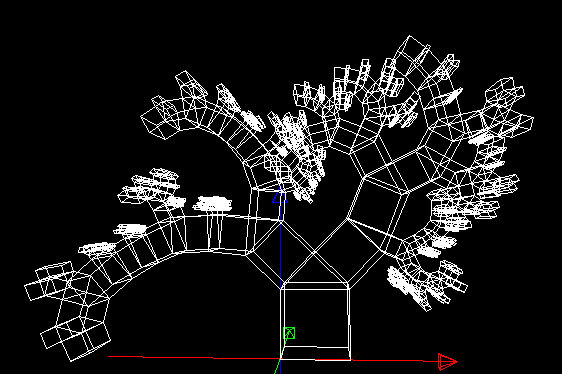
\includegraphics[width=\linewidth]{./pictures/seriell_randomWinkel_Depth8.PNG}
    \captionof{figure}{Pythagoras-Baum mit zufälligen Winkeln.\\Ebenen: 8}
    \label{fig:BaumRandomAngle}
\end{minipage}
\hfill
\begin{minipage}{0.45\linewidth}
    \centering
    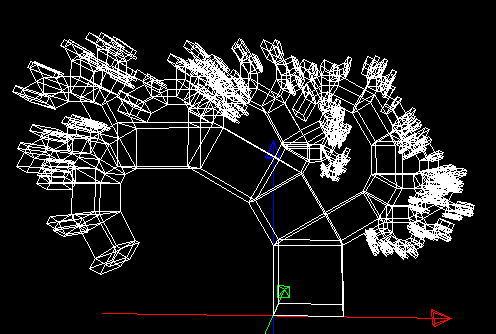
\includegraphics[width=\linewidth]{./pictures/seriell_randomHeight_Depth8.PNG}
    \captionof{figure}{Pythagoras-Baum mit zufälligen Quadern.\\Ebenen: 8}
    \label{fig:BaumRandomHeight}
\end{minipage}

\vspace{0.25cm}
\noindent
Besonders vielfältige Ergebnisse lassen sich erzielen, wenn man zufällige Winkel und zufällige Höhen kombiniert:
\vspace{0.1cm}\\
\noindent
\begin{minipage}{0.45\linewidth}
    \centering
    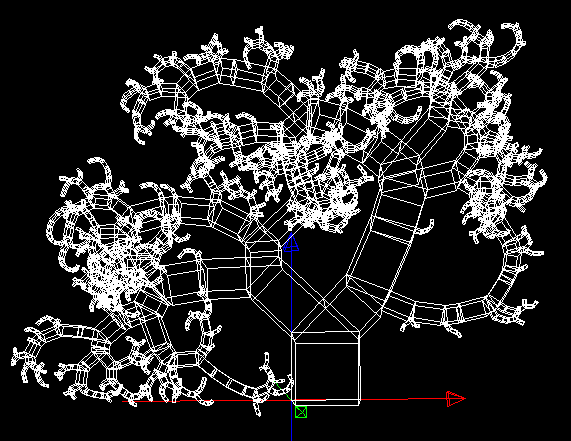
\includegraphics[width=\linewidth]{./pictures/Seriell-random_0.1.PNG}
    \captionof{figure}{Randomisierter Pythagoras-Baum. \\Minmale Seitenlänge: 0.1}
    \label{fig:BaumRandom1}
\end{minipage}
\hfill
\begin{minipage}{0.45\linewidth}
    \centering
    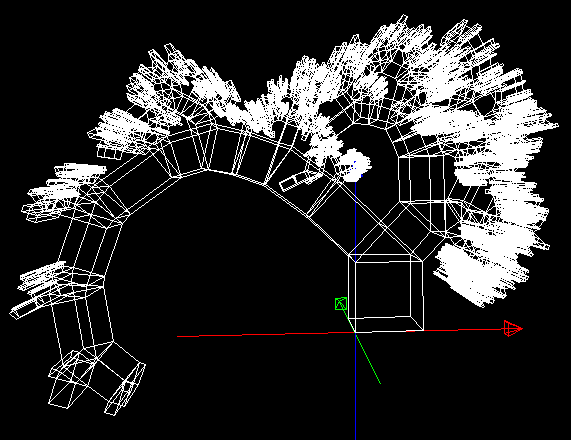
\includegraphics[width=\linewidth]{./pictures/seriell-random_Depth12.PNG}
    \captionof{figure}{Randomisierter Pythagoras-Baum.\\Ebenen: 12}
    \label{fig:BaumRandom2}
\end{minipage}